\documentclass[a5paper,10pt]{article}
 
\usepackage{extsizes}
\usepackage{cmap}
\usepackage[T2A]{fontenc}
\usepackage[utf8x]{inputenc}
\usepackage[english, russian]{babel}

\usepackage{misccorr}

%%%%%%%%%%%%%%%%%%%%%%%%%%%%%%%%%%%%%%%%%%%%%%%%%%%%%%%%%%%%%%%%%%%%%%%%%%%%%%%%%%  
\usepackage{graphicx} % для вставки картинок
\graphicspath{{img/}}
\usepackage{amssymb,amsfonts,amsmath,amsthm} % математические дополнения от АМС

% \usepackage{fontspec}
% \usepackage{unicode-math}

\usepackage{indentfirst} % отделять первую строку раздела абзацным отступом тоже
\usepackage[usenames,dvipsnames]{color} % названия цветов
\usepackage{makecell}
\usepackage{multirow} % улучшенное форматирование таблиц
\usepackage{ulem} % подчеркивания
\linespread{1.3} % полуторный интервал
% \renewcommand{\rmdefault}{ftm} % Times New Roman (не работает)
\frenchspacing
\usepackage{geometry}
\geometry{left=1cm,right=1cm,top=2cm,bottom=1cm,bindingoffset=0cm}
\usepackage{titlesec}
\usepackage{float}
% \definecolor{black}{rgb}{0,0,0}
% \usepackage[colorlinks, unicode, pagecolor=black]{hyperref}
% \usepackage[unicode]{hyperref} %ссылки
\usepackage{fancyhdr} %загрузим пакет
\pagestyle{fancy} %применим колонтитул
\fancyhead{} %очистим хидер на всякий случай
\fancyhead[LE,RO]{Сарафанов Ф.Г.} %номер страницы слева сверху на четных и справа на нечетных
\fancyhead[CO, CE]{Механика}
\fancyhead[LO,RE]{№1.65 -- Иродов И.Е.} 
\fancyfoot{} %футер будет пустой
% \fancyfoot[CO,CE]{\thepage}
\renewcommand{\labelenumii}{\theenumii)}
\newcommand{\ddt}{$\ \pm\ 0.2\ \text{с}$}
\newcommand{\ddtv}{$\ \pm\ 0.8\ \text{с}$}
\newcommand{\ddh}{$\ \pm\ 0.1\ \text{см}$}

\usepackage{amsthm}
\newtheorem{define}{Определение}
\newtheorem{theorem}{Теорема}
\newtheorem{problem}{Задача}

\usepackage{tikz}
\usetikzlibrary{scopes}

\begin{document}

\def\iangle{35} % Angle of the inclined plane

\def\down{-90}
\def\arcr{0.5cm} % Radius of the arc used to indicate angles
\begin{figure}[tb]
	\centering
\begin{tikzpicture}[
    force/.style={>=latex,draw=blue,fill=blue},
    axis/.style={densely dashed,gray,font=\small},
    M/.style={rectangle,draw,fill=lightgray,minimum size=0.5cm,thin},
    m/.style={rectangle,draw=black,fill=lightgray,minimum size=0.3cm,thin},
    plane/.style={draw=black,fill=blue!10},
    string/.style={draw=black, thick},
    pulley/.style={thick},
]

\matrix[column sep=1cm] {
    %% Sketch
    \draw[plane] (0,-1) coordinate (base)
                     -- coordinate[pos=0.5] (mid) ++(\iangle:3) coordinate (top)
                     |- (base) -- cycle;
    \path (mid) node[M,rotate=\iangle,yshift=0.25cm] (M) {};
    \draw[pulley] (top) -- ++(\iangle:0.25) circle (0.25cm)
                   ++ (90-\iangle:0.5) coordinate (pulley);
    \draw[string] (M.east) -- ++(\iangle:1.5cm) arc (90+\iangle:0:0.25)
                  -- ++(0,-1) node[m]  {};

    \draw[->] (base)++(\arcr,0) arc (0:\iangle:\arcr);
    \path (base)++(\iangle*0.5:\arcr+5pt) node {$\alpha$};
    %%

&
    %% Free body diagram of M
    \begin{scope}[rotate=\iangle]
        \node[M,transform shape] (M) {};
        % Draw axes and help lines

        {[axis,->]
            \draw (0,-1) -- (0,2) node[right] {$+y$};
            \draw (M) -- ++(2,0) node[right] {$+x$};
            % Indicate angle. The code is a bit awkward.

            \draw[solid,shorten >=0.5pt] (\down-\iangle:\arcr)
                arc(\down-\iangle:\down:\arcr);
            \node at (\down-0.5*\iangle:1.3*\arcr) {$\alpha$};
        }

        % Forces
        {[force,->]
            % Assuming that Mg = 1. The normal force will therefore be cos(alpha)
            \draw (M.center) -- ++(0,{cos(\iangle)}) node[above right] {$\vec{N}$};
            \draw (M.west) -- ++(-1,0) node[left] {$\vec{f_R}$};
            \draw (M.east) -- ++(1,0) node[above] {$\vec{T}$};
        }

    \end{scope}
    % Draw gravity force. The code is put outside the rotated
    % scope for simplicity. No need to do any angle calculations. 
    \draw[force,->] (M.center) -- ++(0,-1) node[below] {$M\vec{g}$};
    %%

&
    %%%
    % Free body diagram of m
    \node[m] (m) {};
    \draw[axis,->] (m) -- ++(0,-2) node[left] {$+x$};
    {[force,->]
        \draw (m.north) -- ++(0,1) node[above] {$\vec{T'}$};
        \draw (m.south) -- ++(0,-1) node[right] {$m\vec{g}$};
    }

\\
};
\end{tikzpicture}	
\end{figure}

\def\N{\vec{N}}
\def\T{\vec{T}}
\def\t{\vec{T'}}
\def\F{\vec{f_R}}
\def\P{M\vec{g}}
\def\p{m\vec{g}}

Запишем второй закон Ньютона для груза $M$ и $m$: 
\begin{gather}
	M\vec{a}=\N+\T+\F+\P\\
	m\vec{a}=\t+\p
\end{gather}
Учитывая, что нить идеальная  (отсюда $|\T|=|\t|$, $a_m=a_M$), запишем проекции на $x$: 
\begin{gather}
	\label{eq1}Ma=T-\mu{N}-Mg\sin(\alpha)\\
	\label{eq2}ma=mg-T
\end{gather}
И проекция на $y$:
\begin{gather}
	\label{eq3}N=Mg\cos(\alpha)
\end{gather}
Решив систему (\ref{eq1}), (\ref{eq2}), (\ref{eq3}) относительно $a$, получаем
\begin{gather}
	\label{eq4}a=g\frac{(1-(\mu\cos{\alpha}+\sin{\alpha})\frac{M}{m})}{\frac{M}{m}+1}
\end{gather}
Рассматривая знакопеременность числителя дроби в (\ref{eq4}), легко показать, что тогда 
\begin{gather}
	a>0, \hspace{1em}\text{если}\hspace{1em} \frac{m}{M}>\mu\cos{\alpha}+\sin{\alpha}\\
	a<0, \hspace{1em}\text{если}\hspace{1em} \frac{m}{M}<-\mu\cos{\alpha}+\sin{\alpha}
\end{gather}

\end{document}


\begin{document}
% \pagestyle{empty}
% \thispagestyle{empty}
\begin{figure}[H]
	\centering
	\vspace{-1em}
	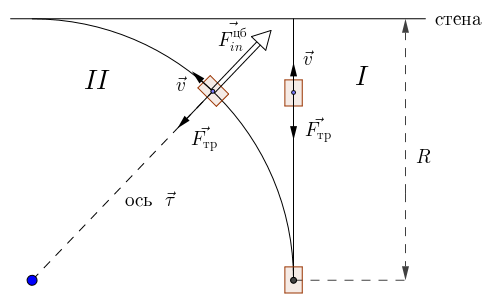
\includegraphics[width=0.96\textwidth]{269-2.png}
	% \caption{Caption }
	% \label{fig:figure1}
\end{figure}
\textbf{Случай $I$.} Рассмотрим движение с торможением без поворота. В проекции на перпендикуляр к стене:

$v=v_0+at$, по 2 закону Ньютона $ma=-F_\text{тр}$, $a=-g\mu$. Тогда можем найти время до остановки $t^*$:
\vspace{-1em}
$$v_\text{ост}=0=v_0-g\mu{}t^* \Longrightarrow t^*=\frac{v_0}{g\mu}$$
% \vspace{-1em}
Тогда из уравнения движения находим пройденное до остановки расстояние $R$:
% \vspace{-0.5em}
$$R=v_0\cdot{t^*}+\frac{a{t^*}^2}{2}=\frac{v_0^2}{g\mu}-\frac{g\mu{}v_0^2}{2(g\mu)^2}=\frac{v_0^2}{2g\mu}$$
% \vspace{-1em}

\textbf{Случай $II$.} Перейдем в НИСО, связанную с автомобилем. НИСО тогда вращается с $\omega=v/r$, а 2 зн. Ньютона запишется как $m\vec{a}'=0=\vec{F}_\text{тр}+\vec{F_{in}^\text{цб}}$. В проекции на $\tau$: $m\omega^2R=g\mu$, Отсюда $$R=\frac{v^2}{g\mu}$$.
\\

\textbf{Вывод.} Торможение без поворота позволит остановится вдвое раньше, чем поворот без торможения и заноса.

\end{document}